%%%%%%%%%%%%%%%%%%%%%%%%%%%%%%%%%%%%%%
%         PACKAGES INCLUSION         %                                                                                      % PACKAGES
%%%%%%%%%%%%%%%%%%%%%%%%%%%%%%%%%%%%%%

\documentclass{article}                                                                                                     % Document specs
\usepackage[legalpaper, margin=2cm]{geometry}                                                                               % Document margin
\usepackage[utf8]{inputenc}                                                                                                 % Encoding specs
\usepackage{tocloft}                                                                                                        % Package import for table of contents with dots
\usepackage{hyperref}                                                                                                       % Package import for external references
\usepackage{graphicx}                                                                                                       % Package import to manage images labels and captions
\usepackage{cite}                                                                                                           % Package import for bibliographies (citations)

%%%%%%%%%%%%%%%%%%%%%%%%%%%%%%%%%%%%%%
%           PREAMBLE START           %                                                                                      % PREAMBLE
%%%%%%%%%%%%%%%%%%%%%%%%%%%%%%%%%%%%%%

\setlength{\parindent}{0em}                                                                                                 % Remove indentation at paragraph's start
\hypersetup{colorlinks=true, linkcolor=red, urlcolor=blue}                                                                  % External references definition: red links and blue URLs (\href call)
\renewcommand{\cftsecleader}{\cftdotfill{\cftdotsep}}                                                                       % Configure table of contents to display dots
\bibliographystyle{plain}                                                                                                   % Bibliography style (plain standard style)

\title{Dijkstra's algorithm implementation \\                                                                               % Title definition (printed with \maketitle command)
\large C project - G3 n.3, numerical calc and programming [145725] AY 2020/2021}                                            % Subtitle definition (printed with \maketitle command)
\author{Cristian Merli, id. 211384}                                                                                         % Authors definition (printed with \maketitle command)
\date{20/07/2021}                                                                                                           % Date definition (printed with \maketitle command)

%%%%%%%%%%%%%%%%%%%%%%%%%%%%%%%%%%%%%%
% END OF PREAMBLE and DOCUMENT START %                                                                                      % DOC-START
%%%%%%%%%%%%%%%%%%%%%%%%%%%%%%%%%%%%%%

\begin{document}                                                                                                            % Document-start

\maketitle                                                                                                                  % Plot previously defined title

\vspace{1cm}                                                                                                                % Vertical-space command
  \begin{abstract}                                                                                                          % Abstract creation
    \noindent \textit{C-code implementation of Dijkstra's algorithm, inside a dedicated library to manage graphs.           % Abstract text
    This library has also been extended so that a graph's structure could be allocated inside heap to test
    Dijkstra’s algorithm. With the aim of getting a more user-friendly output, gnuplot takes care of plotting graphics
    to show the structure of the graph and the elaborated shortest path.}
  \end{abstract}                                                                                                            % Abstract end
\vspace{3.5cm}                                                                                                              % Vertical-space command

\vspace{3.5cm}                                                                                                              % Vertical-space command
  \tableofcontents                                                                                                          % Plot table of contents
\pagebreak                                                                                                                  % Go to new page

\section{Project request}                                                                                                   % Section creation: "Project request"
\label{sec:project_request}                                                                                                 % "project_request" reference-label definition
  Dijkstra. Write a software which reads a graph and given two nodes, calculates the minimum path with Dijkstra’s           % Section text
  algorithm.

\section{Introduction}                                                                                                      % Section creation: "Introduction"
\label{sec:introduction}                                                                                                    % "introduction" reference-label definition
  This document has the main purpose of giving an overview of the project, deeping into theoretical aspects of              % Section text
  Dijkstra's algorithm and how it has been implemented in C-code. While to have further details about technical
  aspects, there is the possibility to consult html documentation of the software (see '\textbf{Doxygen html
  documentation}' section inside '\textbf{README.md}' file).

\section{Dijkstra's algorithm}                                                                                              % Section creation: "Dijkstra's algorithm"
\label{sec:dijkstra_algorithm}                                                                                              % "dijkstra_algorithm" reference-label definition
  Dijkstra's algorithm has been conceived in 1956, by a Dutch computer sientist called Edsger Wybe Dijkstra. The algorithm  % Section text
  is capable of \textbf{finding shortest path between two nodes (source and destination)}, inside a graph data structure.
  It has numerous applications in different fields: from gps-navigation route planning (A* search), electrical/pipelines
  grids design, social networks suggestions, to AI applications as 'best-first search' (uniform cost search). This
  algorithm can be implemented in many different ways, adopting various data-structures and it comes in countless
  variants. In presented c-code library it has been chosen to take advantage of arrays, as data storing-structures.
  While as far as the algorithm itself is concened, it has been implemented in a variant to produce a shortest-path
  tree from source node, to all other nodes inside nodes collection-vector. That allows to be able to re-calculate
  more min-cost paths towards other nodes, without the need of running the algorithm again, if the source node
  remains unvaried.

\section{Graph data-structure}                                                                                              % Section creation: "Graph data-structure"
\label{sec:graph_data_structure}                                                                                            % "graph_data_structure" reference-label definition
  As mentioned in the abstract, graph-library does not contain only Dijkstra’s algorithm, but also a set of functions       % Section text
  to allow graph data-structure \textbf{[}Figure \ref{fig:graph}\textbf{]} management \textit{(for further technical
  details, see doxygen html documentation)}. As briefly touched upon in previous chapter
  \textbf{[}Chapter \ref{sec:dijkstra_algorithm}\textbf{]}, for the purpose of storing \textbf{arches} and \textbf{nodes},
  dynamic-memory vectors have been chosen. The major benefit of that consists of being able to resize the graph during
  runtime, adding or removing elements in allocated memory (\textbf{nodes and arches collection-vectors inside heap}).
  Regarding arches and nodes, they are structure mainly made up of pointers to memory cells of connected elements, in
  addition to element-name and eventual cost. Besides, nodes also have an additional pointer to an element of
  \textbf{dijkstra-dataset dynamic-memory vector}, which contains a set of informations on which Dijkstra's algorithm
  works on. In this way, once the algorithm has been executed, it is possible to recontruct the shortest path backwards
  (from destination to source node), then to be later turned into a forward-path.
  \begin{figure}[ht!]                                                                                                       % Figure-start
    \centering                                                                                                              % Center image
    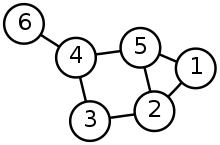
\includegraphics[width=0.25\textwidth]{imgs/graph.png}                                                                  % Size: 25% width of the text
    \caption{\textit{source \href{https://en.wikipedia.org/wiki/Graph_theory}{www.wikipedia.org}}}                          % Image caption
    \label{fig:graph}                                                                                                       % Reference-label to image
  \end{figure}                                                                                                              % Figure-end

\section{Gnuplot}                                                                                                           % Section creation: "Gnuplot"
\label{sec:gnuplot}                                                                                                         % "gnuplot" reference-label definition
  In order to get a more user-friendly output, gnuplot has been integrated in software to draw graph's graphics. More       % Section text
  specifically, two gnuplot scripts are called and loaded from main-testing software, using system commands. The former
  loads data from three static (.dat) files, to \textbf{print the strcture of the graph}
  \textbf{[}Figure \ref{fig:gnuplot1}\textbf{]}; while the latter takes care of plotting loaded data from four
  dynamic (.dat) files, to \textbf{draw graph-structure and highlighting the detected shortest path}
  \textbf{[}Figure \ref{fig:gnuplot2}\textbf{]}. Dynamic-data files are manipulated by main-testing software,
  picking min-cost path plotting informations from the static files (targeting arches/nodes names of the shortest
  path inside files, to copy them).

\section{Library testing}                                                                                                   % Section creation: "Library testing"
\label{sec:library_testing}                                                                                                 % "library_testing" reference-label definition
  It is possible to test graph-library and Dijkstra's algorithm, through the developed main code (graph-test). In order     % Section text
  to that, it creates a test-graph structure to try out and test graph-library. The first stage in graph creation,
  consists in arches and nodes allocation inside heap (names and costs dynamically taken from two vectors, containing
  streets and crosses info to make the example of a road network). During second stage, arches and nodes (streets and
  crosses) are connected together forming a graph-structure \textbf{[}Chapter \ref{sec:graph_data_structure}\textbf{]}.
  Then, once the structure has been created, testing software will ask the user to choose which testing option to adopt.
  There are two different testing options:
  \begin{itemize}                                                                                                           % List start code
    \item \textbf{Prepared test:}                                                                                           % List elements
    calculate shortest path using Dijkstra's algorithm, from pre-defined source to pre-defined destination nodes.
    \item \textbf{Personalized test:}
    calculate shortest path using Dijkstra's algorithm, from specified source to specified destination nodes.
  \end{itemize}                                                                                                             % List end code
  After having the testing-mode choice carried out, the first gnuplot script \textbf{[}Chapter \ref{sec:gnuplot}\textbf{]}
  will graphically display the allocated structure, to give the user a brief overview of the created network. By closing
  this screen, the user can proceed in selected testing mode. Consequently, Dijkstra's algorithm
  \textbf{[}Chapter \ref{sec:dijkstra_algorithm}\textbf{]} will be applied to detect all the min-cost paths, then
  reconstructing the specifically requested one. Here the second gnuplot script
  \textbf{[}Chapter \ref{sec:gnuplot}\textbf{]} will be called aiming to display the allocated graph (gray coloured),
  highlighting the elaborated shortest path between source and destination nodes (specified during tesing option choice).
  After graphical representation is closed, the whole structure and all the dynamic memory allocated inside heap, will
  be cleared immediately before closing test software.

\section{Conclusions}                                                                                                       % Section creation: "Conclusions"
\label{sec:conclusions}                                                                                                     % "conclusions" reference-label definition
  To sum up, in this particular test, Dijkstra’s algorithm has been implemented to find shortest path between two crosses   % Section text
  inside a road network, but the \textbf{library can be utilized in very different applications} thanks to the importance
  of the algorithm itself. That's because it still remains one of the best and most diffused algorithms in all its
  variants, to find shortest paths from a single-source node inside a graph. To conclude with a citation, ”The Dijkstra’s
  algorithm has its own shortcomings when seeking an optimal path between two points, but it has irreplaceable
  advantages.” \textit{(by DongKai Fan, Ping Shi)}
  \cite{5569452}                                                                                                            % Bibliography cit.

\section{Images}                                                                                                            % Section creation: "Images"
\label{sec:images}                                                                                                          % "images" reference-label definition
  \begin{figure}[ht!]                                                                                                       % Figure-start
    \centering                                                                                                              % Center image
    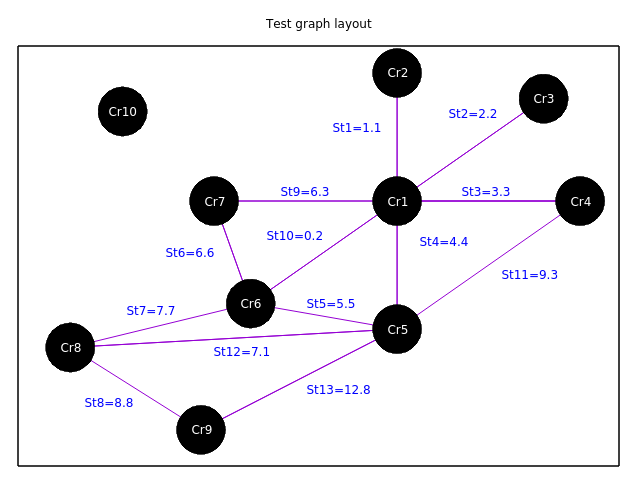
\includegraphics[width=0.65\textwidth]{../../sw/gnuplot/exports/imgs/test_graph.png}                                    % Size: 65% width of the text
    \caption{\textit{Graph-structure (exported from gnuplot)}}                                                              % Image caption
    \label{fig:gnuplot1}                                                                                                    % Reference-label to image
  \end{figure}                                                                                                              % Figure-end
  \begin{figure}[ht!]                                                                                                       % Figure-start
    \centering                                                                                                              % Center image
    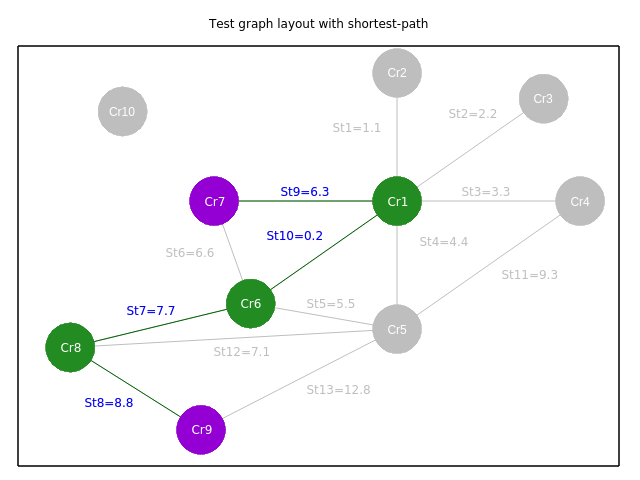
\includegraphics[width=0.65\textwidth]{../../sw/gnuplot/exports/imgs/personalized_shortest_path.png}                    % Size: 65% width of the text
    \caption{\textit{Graph-structure with shortest path between 'Cross9' and 'Cross7' (exported from gnuplot)}}             % Image caption
    \label{fig:gnuplot2}                                                                                                    % Reference-label to image
  \end{figure}                                                                                                              % Figure-end

\bibliography{biblio/references}                                                                                            % Bibliography inclusion (biblio/references.bib)

\end{document}                                                                                                              % End document code

%%%%%%%%%%%%%%%%%%%%%%%%%%%%%%%%%%%%%%
%            DOCUMENT END            %                                                                                      % DOC-END
%%%%%%%%%%%%%%%%%%%%%%%%%%%%%%%%%%%%%%
